\begin{itemize}
    \item Triangle centers
    \item Are Loci Algebraic (method of resultants, why so many)
    \item Are Loci Elliptic (Blaschke's parametrization \cite{daepp-2019})
    \item Monotonicity and Turning Number (ballet + paper 25)
    \item Table of results
    \item A list of the elliptic loci of centers in the $X_{1}$ to $X_{200}$ range can be found \href{https://dan-reznik.github.io/why-so-many-ellipses/}{here}.
\end{itemize}

\subsection{Generic Nested Ellipses}
 
 In this Section we prove the locus of a given fixed linear combination of $X_2$ and $X_3$ is an ellipse. We will continue to use Blaschke product techniques since a generic non-concentric pair can always be seen as the affine image of a pair with circumcircle.

\begin{figure}
    \centering
    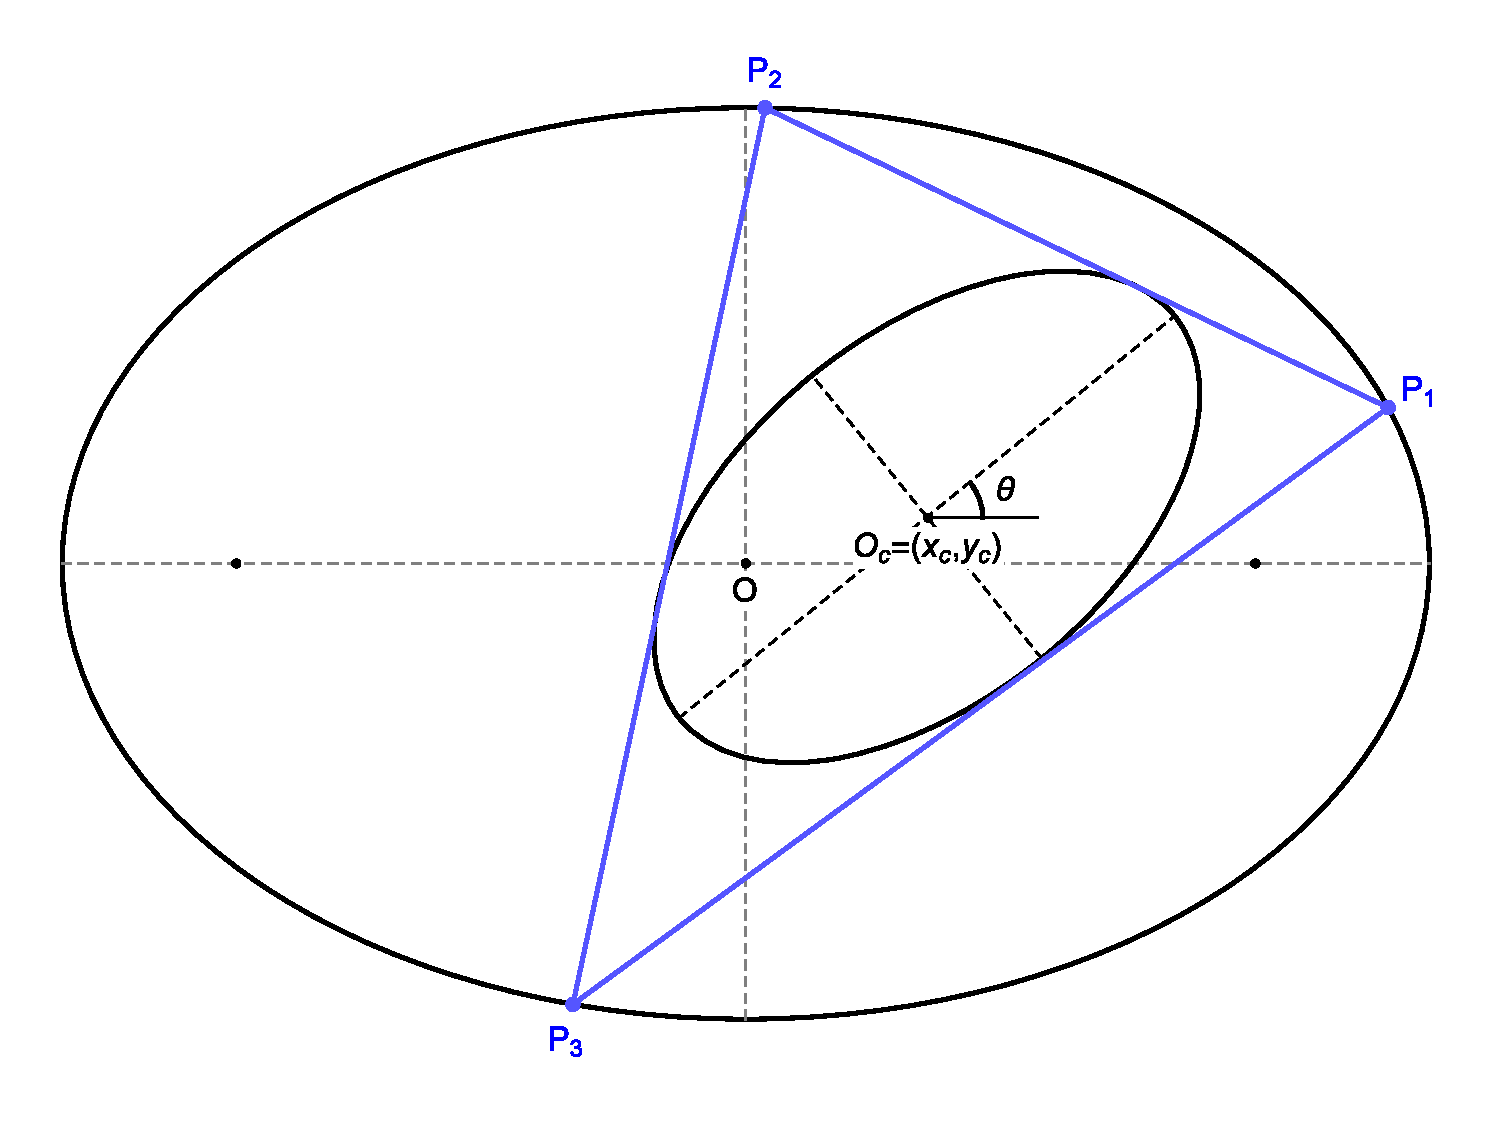
\includegraphics[width=.8\textwidth]{pics_04_010_n3_nonconcentric.eps}
    \caption{A pair of ellipses in general position which admits a Poncelet 3-periodic family (blue). Let the outer one be centered at the origin $O$. Their major axes are tilted by $\theta$, and their centers displaced by $O_c=(x_c,y_c)$. \href{https://youtu.be/bjHpXVyXXVc}{Video}}
    \label{fig:04-n3-nonconcentric}
\end{figure}

Consider the generic pair of nested ellipses $\E=(O,a,b)$ and $\E_c=(O_c,a_c,b_c.\theta)$ in Figure~\ref{fig:04-n3-nonconcentric}. Let s$\theta$, c$\theta$ denote the sine and cosine of $\theta$, respectively. Define $c_c^2=a_c^2-b_c^2$. The Cayley condition for the pair to admit a 3-periodic family is given by:

{\small
\begin{align}
&{b}^{4}x_c^{4}+2\,{a}^{2}{b}^{2}x_c^{2}y_c^{2}+
 \left(  2 c_c^2  \left( -{b}^{2}({a}^{2}+{b}^{2} )\right)  \text{c}\theta^2  - 2\left(  \,b ^{2}- \,b_c
^{2} \right) {b}^{2}{a}^{2}-2\,{b}^{4}b_c^{2} \right)x_c
^{2} \label{eqn:cayley}\\
&-8\,{a}^{2}{b}^{2}x_c\,{  y_c}\,c_c^2 
\text{s}\theta\text{c}\theta  +{a}^{4}y_c^{4} + \left(  2 c_c^2 a^2 \left(
{a}^{2}+{b}^{2}  \right)\text{c}\theta^2  
 -2 \left(  \,b_c^{2}+{b}^{2} \right) {a}^{4}+2
\,{a}^{2}{b}^{2}b_c^{2} \right) y_c^{2} \nonumber\\
&+ c_c^4  c^4  \left( \text{c}\theta^4-2\, c_c^2 c^2
  \left( {a}^{2} a_c^{2}-{b}^{2}{a}^{2}+
b_c^{2}{b}^{2} \right) \text{c}\theta^2 \right. \nonumber\\
 &+ \left( a a_c+a b-b b_c \right)  \left( a a_c
-a b -b b_c \right)  \left( a a_c+a b+b b_c \right)  \left( a
a_c-a b+b b_c \right) = 0\nonumber
\end{align}
}


 




Recall that over Poncelet N-periodics interscribed in a generic pair of conics, the locus of vertex and area centroids is an ellipse \cite{sergei2016-com} as is that of the circumcenter-of-mass \cite{sergei2014-circumcenter-of-mass}, a generalization of $X_3$ for $N>3$. Referring to Figure~\ref{fig:nonconcentric-xns}:

\begin{theorem}
Over the family of 3-periodics interscribed in an ellipse pair in general position (non-concentric, non-axis-aligned),
if $\X\ab$ is a fixed linear combination of $X_2$ and $X_3$, i.e., $\X\ab=\alpha X_2+\beta X_3$ for some fixed $\alpha,\beta\in\mathbb{C}$, then its locus is an ellipse. 
\label{thm:ellipse-locus}
\end{theorem}

\begin{proof}
Consider a general $N=3$ Poncelet pair of ellipses that forms a 1-parameter family of triangles. Without loss of generality, by translation and rotation, we may assume the outer ellipse is centered at the origin and axis-aligned with the plane $\R^2$, which we will also identify with the complex plane $\mathbb{C}$. Let $a,b$ be the semi-axis of the outer ellipse, and $a_c,b_c$ the semi-axis of the inner ellipse, as usual. 

Referring to Figure~\ref{fig:affine}, consider the linear transformation that takes $(x,y)\mapsto(x/a,y/b)$. This transformation takes the outer ellipse to the unit circle $\T$ and the inner ellipse to another ellipse. Thus, it transforms the general Poncelet $N=3$ system into a pair where the outer ellipse is the circumcircle, which we can parametrize using Blaschke products \cite{daepp-2019}. In fact, to get back to the original system, we must apply the inverse transformation that takes $(x,y)\mapsto(a x,b y)$. As a linear transformation from $\mathbb{C}$ to $\mathbb{C}$, we can write it as $L(z):=p z+q \ol{z}$, where $p:=(a+b)/2, q:=(a-b)/2$.

\begin{figure}
    \centering
    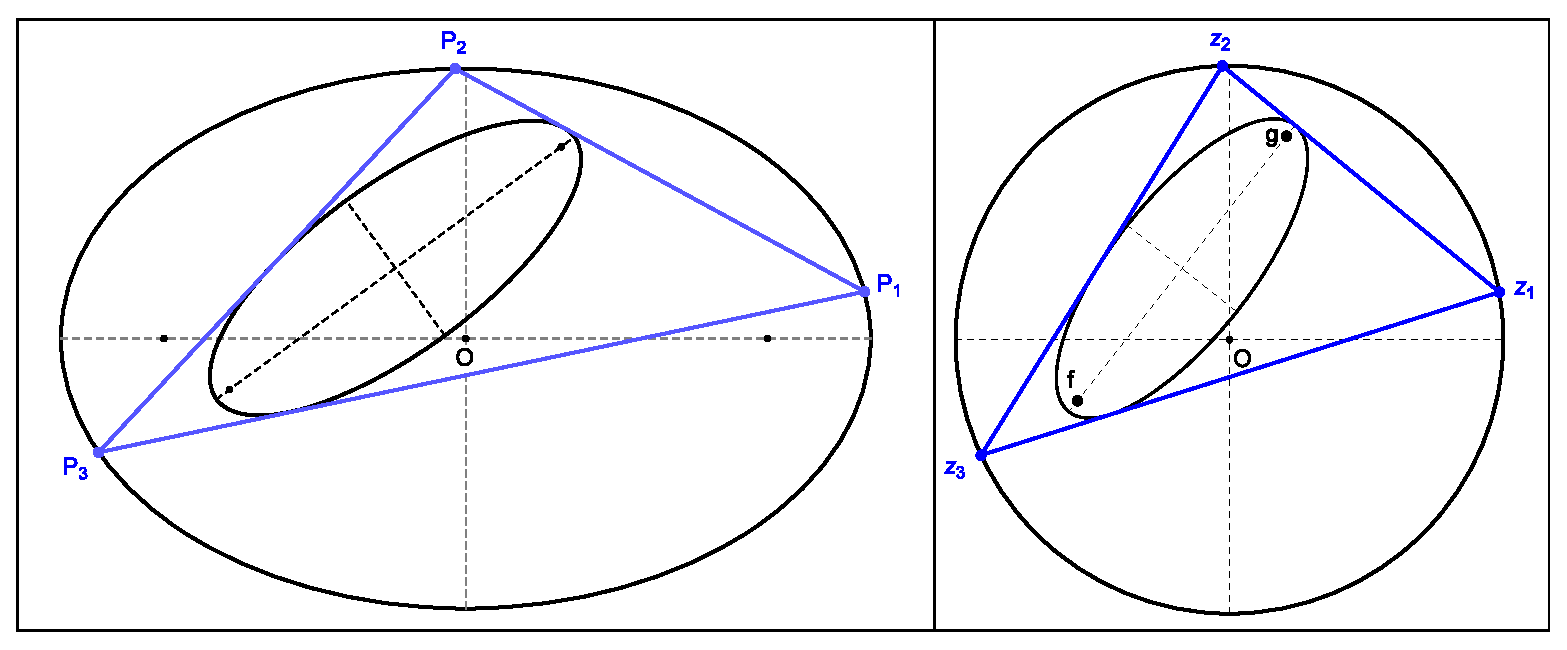
\includegraphics[width=\textwidth]{pics_04_030_affine_circumcircle.eps}
    \caption{Affine transformation that sends a generic ellipse pair and its 3-periodic family (left) to a new pair with circumcircle (right). We parametrize the 3-periodic orbit with vertices $z_i$ in the circumcircle pair using the foci of the latter's caustic $f$ and $g$, and then apply the inverse affine transformation to get a parametrization of the vertices $P_i$ of the original Poncelet pair. \href{https://youtu.be/6xSFBLWIkTM}{Video}}
    \label{fig:affine}
\end{figure}


Let $z_1,z_2,z_3\in\T\subset\mathbb{C}$ be the three vertices of the circumcircle family, parametrized as in Definition~\ref{def:bla}, and let $v_1:=L(z_1),v_2:=L(z_2),v_3:=L(z_3)$ be the three vertices of the original general family. The barycenter $X_2$ of the original family is given by $(v_1+v_2+v_3)/3$, and the circumcenter $X_3$ is given by \cite{stackexchange-x3a}:

\[
    X_3=\left|
        \begin{array}{ccc}
          v_1 & |v_1|^2 & 1 \\
          v_2 & |v_2|^2 & 1 \\
          v_3 & |v_3|^2 & 1
        \end{array}
      \right| \Bigg/
     \left|
        \begin{array}{ccc}
          v_1 & \overline{v_1} & 1 \\
          v_2 & \overline{v_2} & 1 \\
          v_3 & \overline{v_3} & 1
        \end{array}
      \right|
\]

Since $\ol{z_1}=1/z_1,\ol{z_2}=1/z_2,\ol{z_3}=1/z_3$, we can write $v_1,v_2,v_3$ as rational functions of $z_1,z_2,z_3$, respectively. Thus, both $X_2$ and $X_3$ are symmetric rational functions on $z_1,z_2,z_3$. Defining $\X\ab=\alpha X_2+\beta X_3$, we have consequently that $\X\ab$ is also a symmetric rational function on $z_1,z_2,z_3$. Hence, we can reduce its numerator and denominator to functions on the elementary symmetric polynomials on $z_1,z_2,z_3$. This is exactly what we need in order to use the parametrization by Blaschke products.

In fact, we explicitly compute:
\[  \X\ab= \frac{p^2 q \left(\sigma_2 (\alpha +3 \beta )+3 \beta  \sigma_3^2\right)+\alpha  p^3 \sigma_1 \sigma_3-p q^2 (3 \beta +\sigma_1 \sigma_3 (\alpha +3 \beta ))-\alpha  q^3 \sigma_2}{3 \sigma_3 (p-q) (p+q)}\]
where $\sigma_1,\sigma_2,\sigma_3$ are the elementary symmetric polynomials on $z_1,z_2,z_3$.

Let $f,g\in\mathbb{C}$ be the foci of the inner ellipse in the circumcircle system. Using Definition~\ref{def:bla}, with the parameter $\l$ varying on the unit circle $\T$, we get:

\begin{equation}
\X\ab= u \l+v\frac{1}{\l}+w
\label{eqn:xi-param}
\end{equation}

\noindent where:

\begin{align*}
    u:=&\frac{p \left(\ol{f} \ol{g} \left(\alpha  p^2-q^2 (\alpha +3 \beta )\right)+3 \beta  p q\right)}{3 (p-q) (p+q)}\\
    v:=&\frac{\beta  p q (q-f g p)}{(q-p) (p+q)}+\frac{1}{3} \alpha  f g q\\
    w:=&\frac{q \left(\ol{f}+\ol{g}\right) \left(p^2 (\alpha +3 \beta )-\alpha  q^2\right)+p (f+g) \left(\alpha  p^2-q^2 (\alpha +3 \beta )\right)}{3 (p-q) (p+q)}
\end{align*}

By   \cref{lem:ell-param}, this is the parametrization of an ellipse centered at $w$, as desired. As in  \cref{lem:ell-param}, it is also possible to explicitly calculate its axis and rotation angle, but these expressions become very long.
\end{proof}

\begin{corollary}
Over the family of 3-periodics interscribed in an ellipse pair in general position (non-concentric, non-axis-aligned),
if $\X_\gamma$ is a real affine combination of $X_2$ and $X_3$, i.e., $\X_\gamma=(1-\gamma) X_2+\gamma X_3$ for some fixed $\gamma\in\R$, then its locus is an ellipse. Moreover, as we vary $\gamma$, the centers of the loci of the $\X_\gamma$ are collinear.
\end{corollary}

\begin{proof}
Apply   \cref{thm:ellipse-locus} with $\alpha=1-\gamma, \beta=\gamma$ to get the elliptical loci. As in the end of the proof of  \cref{thm:ellipse-locus}, the center of the locus of $\X_\gamma$ can be computed explicitly as 
\begin{gather*}
    w=w_0+w_1 \gamma \text{, where}\\
    w_0=\frac{1}{3} \left(q \left(\ol{f}+\ol{g}\right)+p (f+g)\right)\\
    w_1=\frac{q \left(2 p^2+q^2\right) \left(\ol{f}+\ol{g}\right)-p (f+g) \left(p^2+2 q^2\right)}{3 (p-q) (p+q)}
\end{gather*}
As $\gamma\in\R$ varies, it is clear the center $w$ sweeps a line.
\end{proof}

We proved that all of the following triangle centers have elliptic loci in the general N=3 Poncelet system, including the barycenter, circumcenter, orthocenter, nine-point center, and de Longchamps point (reflection of the orthocenter  about the circumcenter of a triangle):

\begin{observation}
Amongst the 40k+ centers listed on \cite{etc}, about 4.9k triangle centers lie on the Euler line \cite{etc-central-lines}. Out of these, only 226 are fixed affine combinations of $X_2$ and $X_3$. For $k<1000$, these amount to $X_k,k=${\small 2, 3, 4, 5, 20, 140, 376, 381, 382, 546, 547, 548, 549, 550, 631, 
632}.
\label{obs:affine-euler-line}
\end{observation}

\begin{figure}
     \centering
     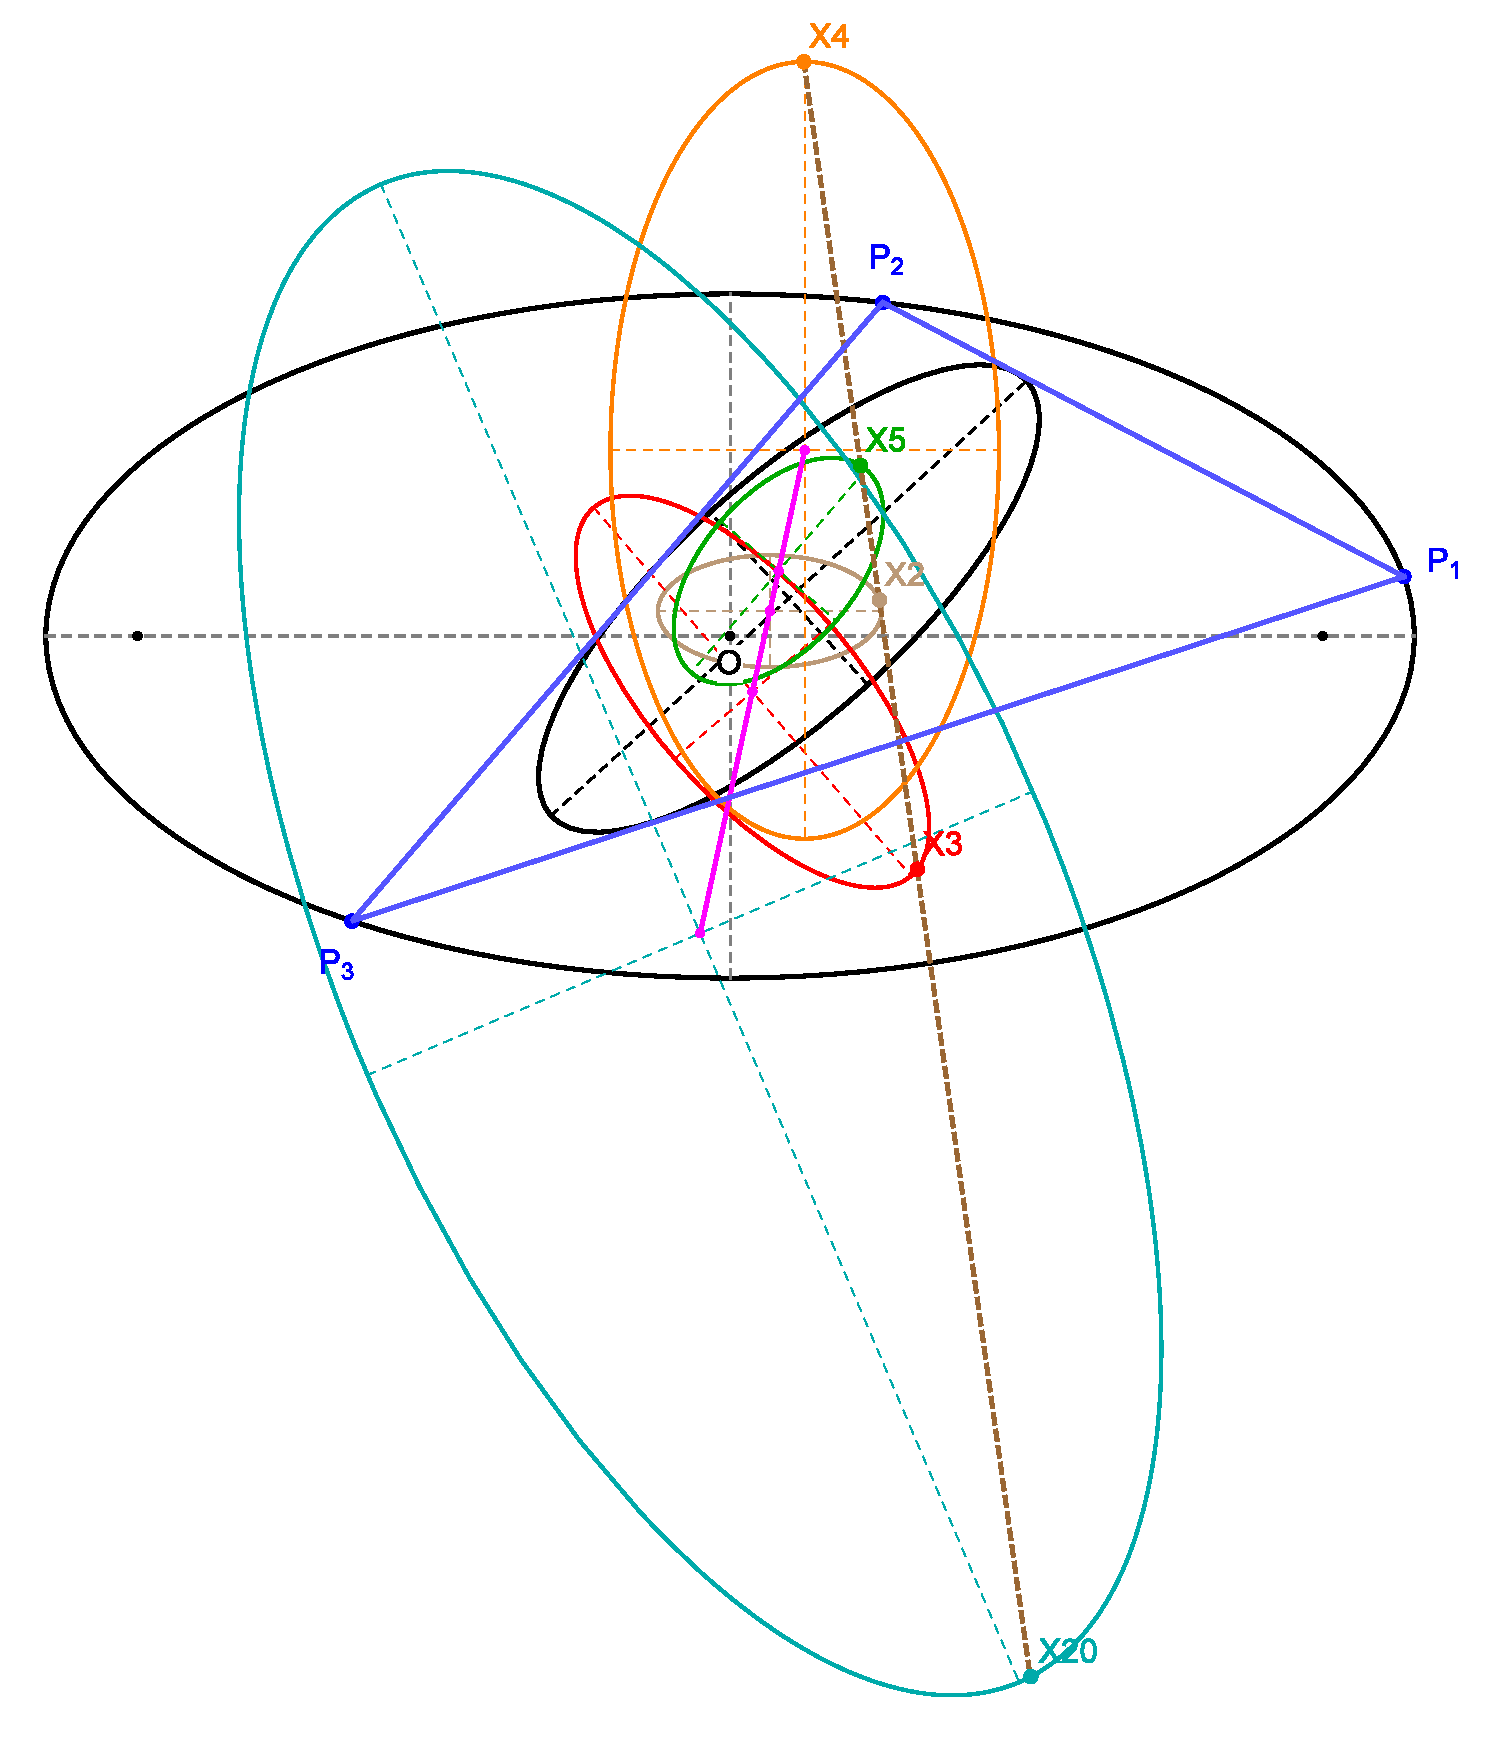
\includegraphics[width=.8\textwidth]{pics_04_020_n3_nonconcentric_loci.eps}
     \caption{A 3-periodic is shown interscribed between two nonconcentric, non-aligned ellipses (black). The loci of $X_k$, $k=2,3,4,5,20$ (and many others) remain ellipses. Those of $X_2$ and $X_4$ remain axis-aligned with the outer one. Furthermore the centers of all said elliptic loci are collinear (magenta line). \href{https://youtu.be/p1medAei_As}{Video}}
     \label{fig:nonconcentric-xns}
 \end{figure}
 
%\begin{corollary}
%The elliptic loci of $X_2$, $X_3$ and $X_4$ are given by:
%\[ \textcolor{red}{mark} \]
%\textcolor{red}{these will be hard to get explicitly}
%\end{corollary}
 
\begin{observation}\label{obs:X2X4}
The elliptic loci of $X_2$ and $X_4$ are axis-aligned with the outer ellipse.
\end{observation} 

We conclude this section with phenomenon specific to the case where $\E_c$ is a circle,  ~\cref{fig:circular-caustic}:

\begin{observation}
 Over the family of 3-periodics inscribed in an ellipse and circumscribing a non-concentric circle centered on $O_c=X_1$, the locus of $X_3$ and $X_5$ are ellipses whose major axes pass through $X_1$.
 \end{observation}
 
\begin{figure}
    \centering
    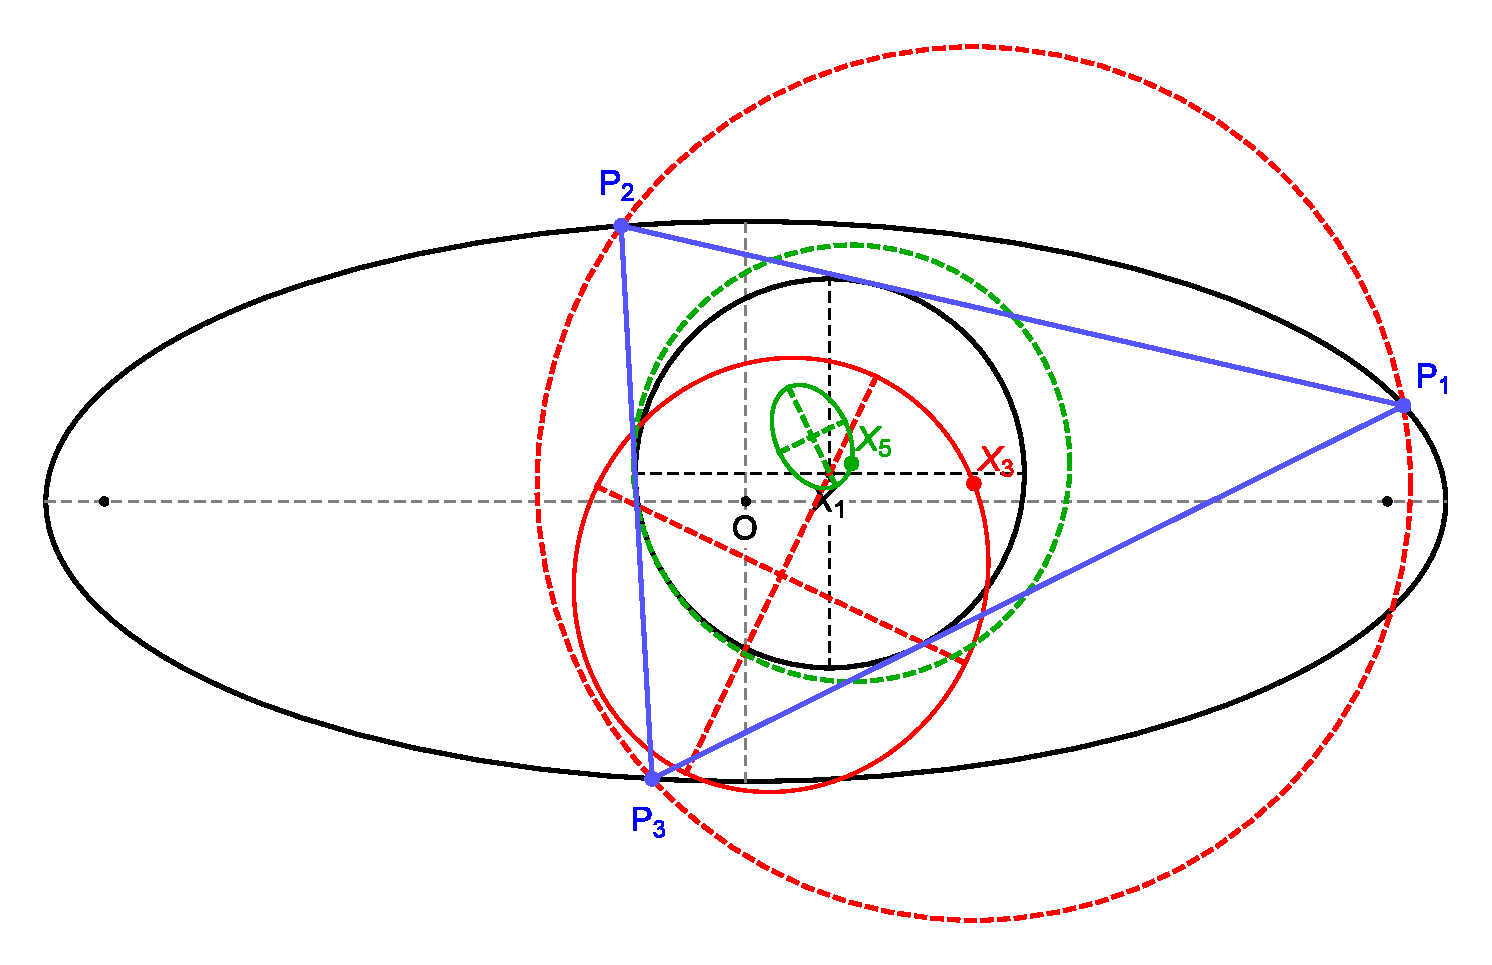
\includegraphics[width=.7\textwidth]{pics_04_040_n3_nonconcentric_circular_caustic.eps}
    \caption{A 3-periodic (blue) is shown inscribed in an outer ellipse and an inner non-concentric circle centered on $O_c$. The loci of both circumcenter (solid red) and Euler center (solid green) are ellipses whose major axes pass through $O_c$. \href{https://youtu.be/w7sZ5O8k4xU}{Video}}
    \label{fig:circular-caustic}
\end{figure}



Referring to Figure~\ref{fig:nonconcentric-circumcircle-circular-loci-right-tris}:

\begin{proposition}
If a triangle center $\X\ab=\alpha X_2+ \beta X_3$ is a fixed linear combination of $X_2$ and $X_3$ for some $\alpha,\beta\in\mathbb{C}$, its locus over 3-periodics in the non-concentric pair with a circumcircle is a circle centered on $\mathcal{O}_\alpha$ and of radius $\mathcal{R}_\alpha$ given by:

\[ \mathcal{O}_\alpha = \frac{\alpha(f+g)}{3},\;\;\; \mathcal{R}_\alpha =\frac{|\alpha f g|}{3}\]
\label{prop:LinComb-concentric}
\end{proposition}

\begin{observation}
Notice that the center and radius of the locus do not depend on $\beta$ since the circumcenter $X_3$ is stationary at the origin of this system.
\end{observation}

\begin{proof}
Since, $z_1,z_2,z_3$ are the 3 vertices of the Poncelet triangle inscribed in the unit circle, its barycenter and circumcenter are given by $X_2=(z_1+z_2+z_3)/3$ and $X_3=0$, respectively. We define $\X\ab:=\alpha X_2+ \beta X_3=\alpha (z_1+z_2+z_3)/3$. Using Definition~\ref{def:bla}, we get $\X\ab=\alpha(f+g+\l \ol{f}\ol{g})/3=\alpha(f+g)/3+\l(\alpha \ol{f}\ol{g})/3$, where the parameter $\l$ varies on the unit circle $\T$. Thus, the locus of $\X_{\gamma}$ over the Poncelet family of triangles is a circle with center $\mathcal{O}_{\alpha}:=\alpha(f+g)/3$ and radius $\mathcal{R}_{\alpha}:=|\alpha \ol{f}\ol{g}|/3=|\alpha f g|/3$.
\end{proof}

Using $\alpha=1-\gamma, \beta=\gamma$ for a fixed $\gamma\in\R$ in   \cref{prop:LinComb-concentric}, we get:

\begin{corollary}
 If a triangle center $\X_\gamma=(1-\gamma) X_2+ \gamma X_3$ is a real affine combination of $X_2$ and $X_3$ for some $\gamma\in\R$, its locus over 3-periodics in the non-concentric pair with a circumcircle is a circle. Moreover, as we vary $\gamma$, the centers of these loci are collinear with the fixed circumcenter.
 \label{cor:gamma-with-circumcircle}
\end{corollary}

Many triangle centers in \cite{etc} are affine combinations of the barycenter $X_2$ and circumcenter $X_3$. See   \cref{obs:affine-euler-line} for a compilation of them.

\begin{observation}
For a generic triangle, only $X_{98}$, and $X_{99}$ are simultaneously on the Euler line and on the circumcircle. However these are not linear combinations of $X_2$ and $X_3$. Still, if a triangle center is always on the circumcircle of a generic triangle (there are many of these, see \cite[Circumcircle]{mw}), its locus over 3-periodics in the non-concentric pair with circumcircle is trivially a circle.
\end{observation}

 
\begin{corollary}
 Over the family of 3-periodics inscribed in a circle and circumscribing a non-concentric inellipse centered at $O_c$, the locus of $X_k$, $k$ in 2,4,5,20 are circles whose centers are collinear. The locus of $X_5$ is centered on $O_c$. The centers and radii of these circular loci are given by:

\begin{alignat*}{4}
    O_2&=\frac{f+g}{3},\quad& O_4&=f+g,\quad&O_5&=\frac{f+g}{2},\quad&O_{20}&=-(f+g)\\
    r_2&=\frac{|f g|}{3},\quad&r_4 &= |f g|,\quad&r_5 &= \frac{|f g|}{2},\quad& r_{20}&= |f g|
\end{alignat*}

\end{corollary}

\begin{proof}
As in  \cref{cor:gamma-with-circumcircle}, we can use  \cref{prop:LinComb-concentric} with $\gamma=0,-2,-1/2,4$ to get the center and radius for $X_2,X_4,X_5,X_{20}$, respectively. All of these centers are real multiples of $f+g$, so they are all collinear. Moreover, the center $O_5$ of the circular loci of $X_5$ is $(f+g)/2$, that is, the midpoint of the foci of the inellipse, or in other words, the center $O_c$ of the inellipse.
\end{proof}
 
Referring to  \cref{fig:nonconcentric-circumcircle-circular-loci-right-tris}:

\begin{observation}
The family of 3-periodics in the pair with circumcircle includes obtuse triangles if and only if $X_3$ is exterior to the caustic. \end{observation}

This is due to the fact that when $X_3$ is interior to the caustic, said triangle center can never be exterior to the 3-periodic. Conversely, if $X_3$ is exterior, it must also be external to some 3-periodic, rendering the latter obtuse.

\begin{figure}
    \centering
    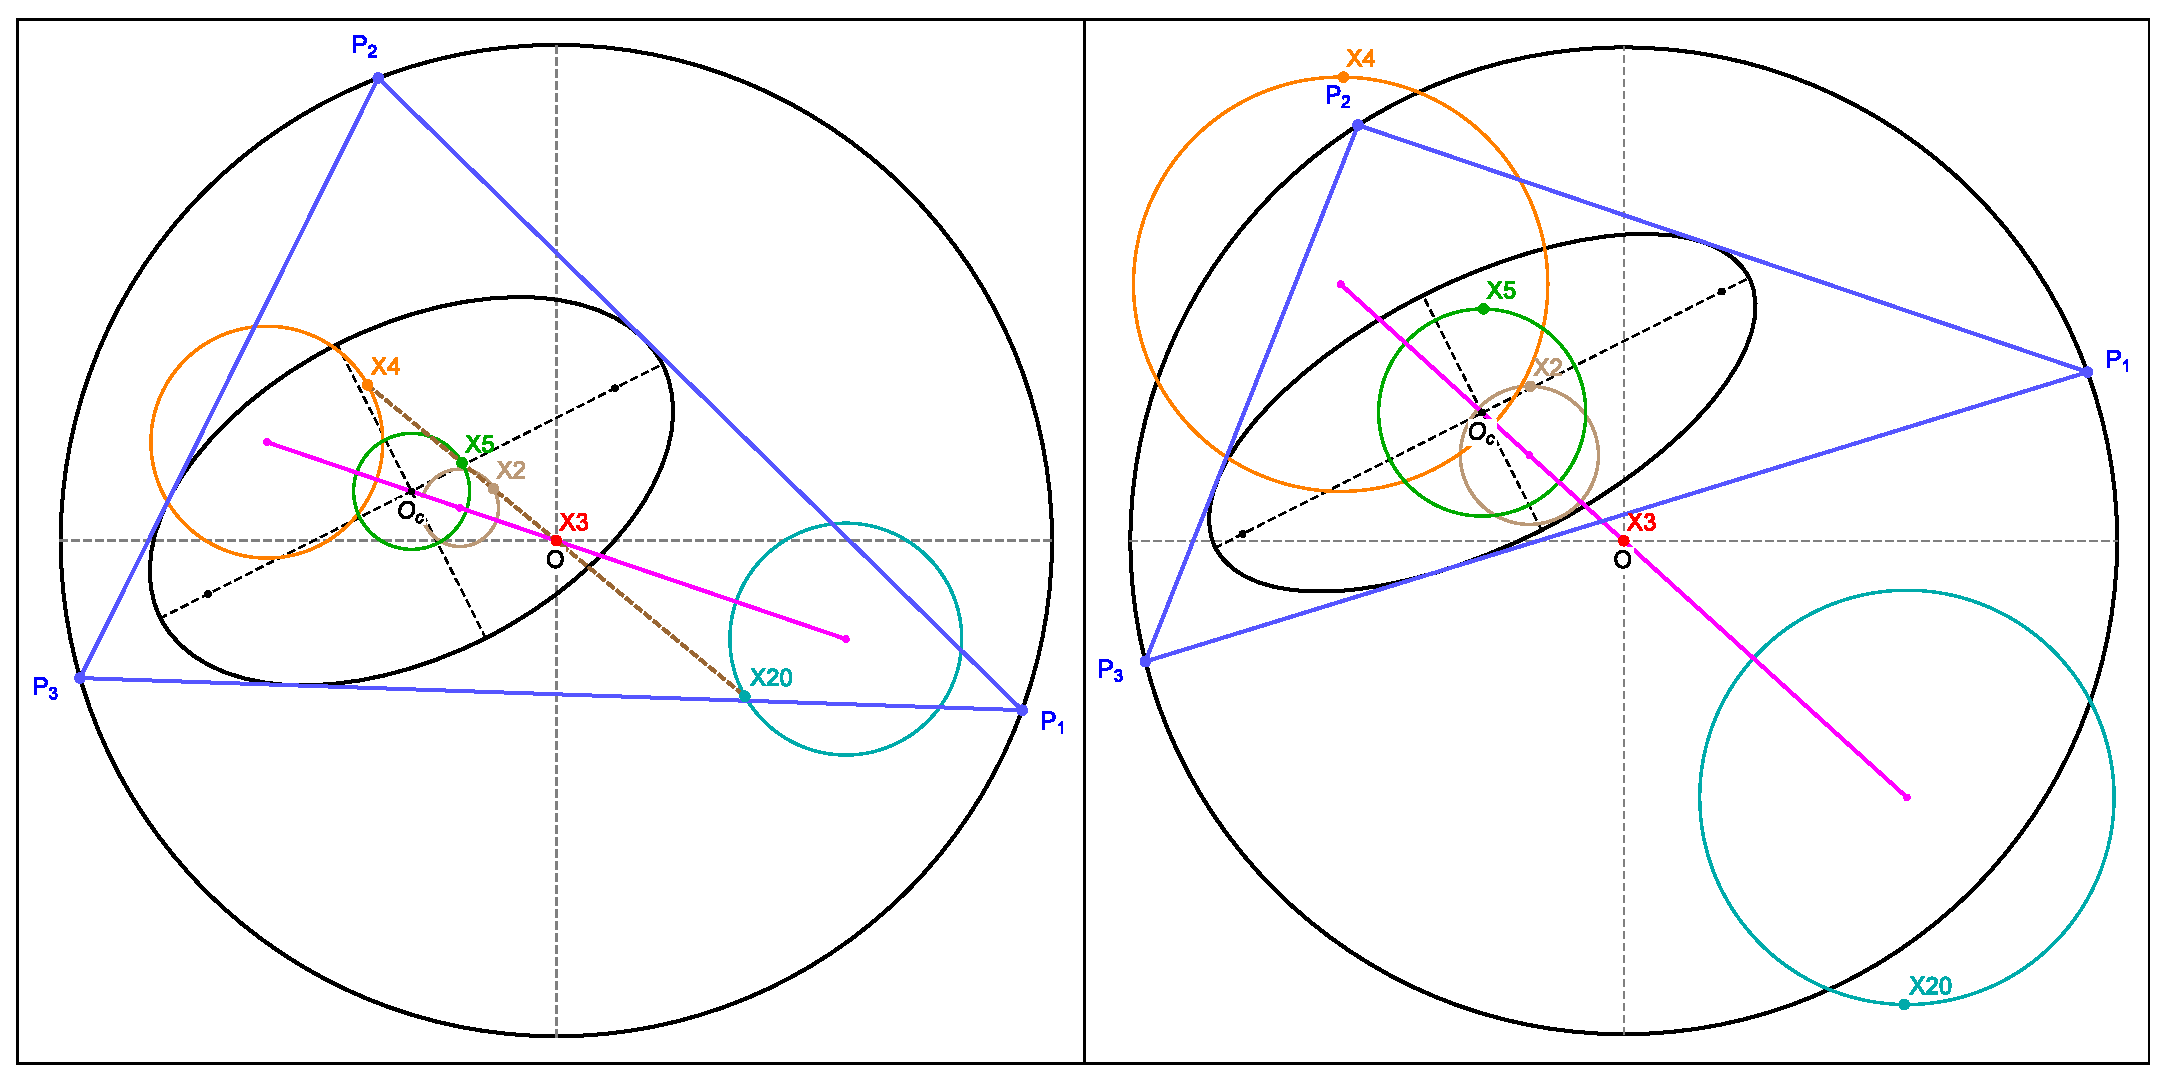
\includegraphics[width=\textwidth]{pics_03_010_n3_circumcircle_pair.eps}
    \caption{\textbf{Left:} 3-periodic family (blue) in the pair with circumcircle where the caustic contains $X_3$, i.e., all 3-periodics are acute. The loci of $X_4$ and $X_{20}$ are interior to the circumcircle. \textbf{Right:} $X_3$ is exterior to the caustic, and 3-periodics can be either acute or obtuse. Equivalently, the locus of $X_4$ intersects the circumcircle. In both cases (left and right), the loci of $X_k$, $k$ in 2,4,5,20 are circles with collinear centers (magenta line). The locus of $X_5$ is centered on $O_c$. The center of the $X_2$ locus is at $2/3$ along $O O_c$. \href{https://youtu.be/HXgJQo2UT_8}{Video}}
    \label{fig:nonconcentric-circumcircle-circular-loci-right-tris}
\end{figure} 


Consider the parametrization of a triangular orbit $\{z_1,z_2,z_3\}$ given in \cref{def:bla}.

Let also the  affine transformation
$T(z)=pz+q\ol z$.

\textcolor{red}{figura do blaschke}

\begin{theorem}
Over the family of 3-periodics interscribed in a generic nested pair of ellipses (non-concentric, non-axis-aligned),
if $\X\ab$ is a fixed linear combination of $X_2$ and $X_3$, i.e., $\X\ab=\alpha X_2+\beta X_3$ for some fixed $\alpha,\beta\in\mathbb{C}$, then its locus is an ellipse. 
\label{thm:ellipse-locus-linear-combination}
\end{theorem}


